%%% Local Variables:
%%% mode: latex
%%% TeX-master: "../main"
%%% End:
\newcommand{\flux}[1]{L_#1(\pmb{x}, \vec{\omega_o})}


\section{Introduction}

\begin{frame}
  \frametitle{Rendering Translucent Materials}
  \only<1>{\begin{figure}[!ht]
    \centering
    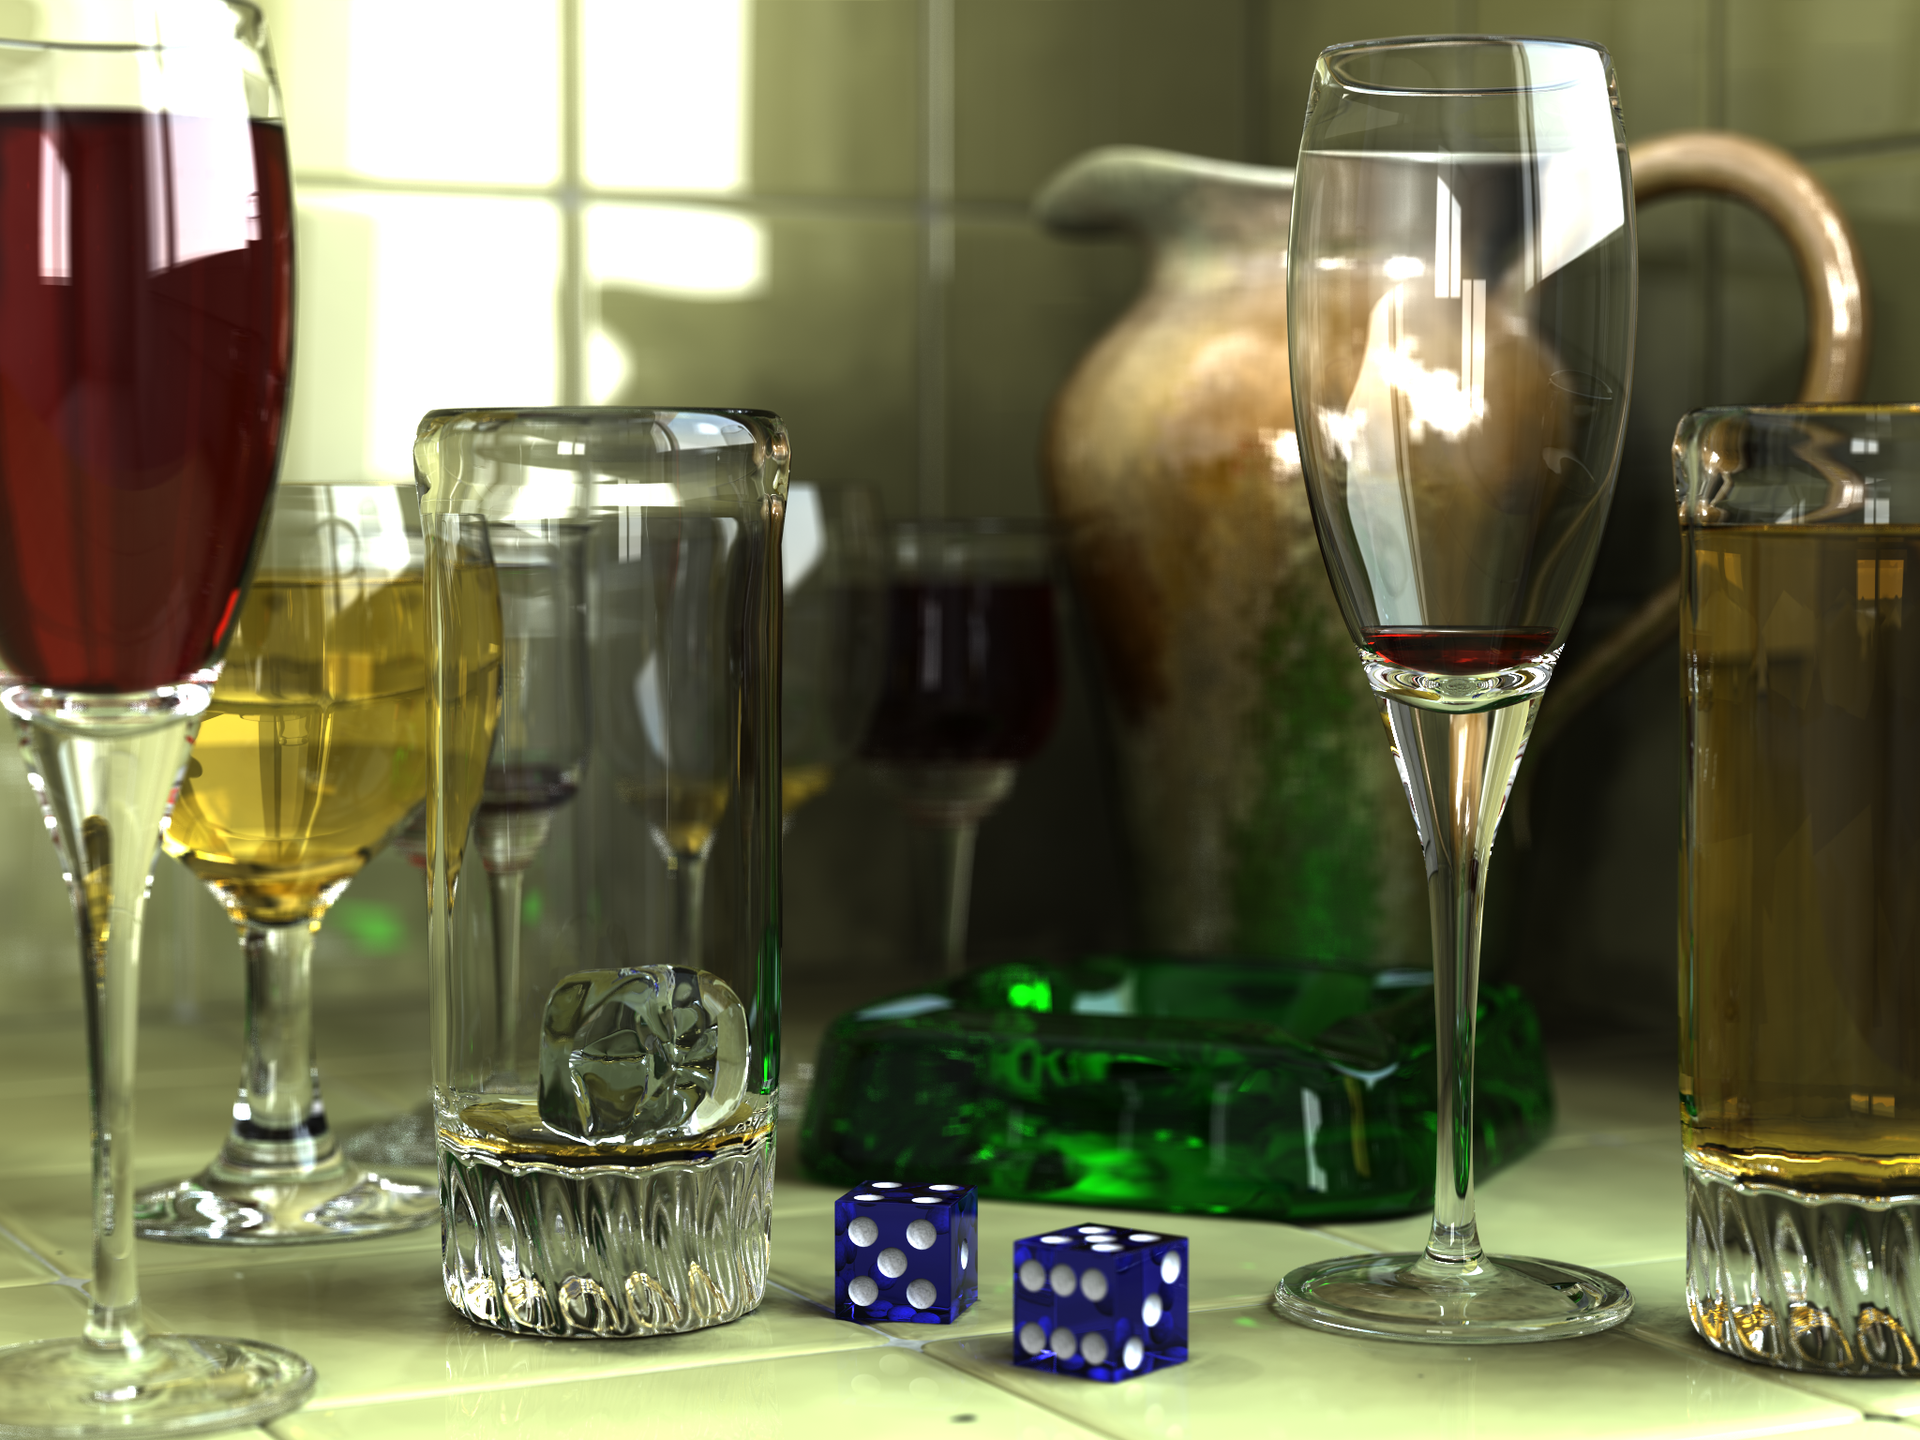
\includegraphics[scale=0.15]{renering.png}
  \end{figure}
}
\only<2>{
  \begin{figure}[!ht]
    \centering
    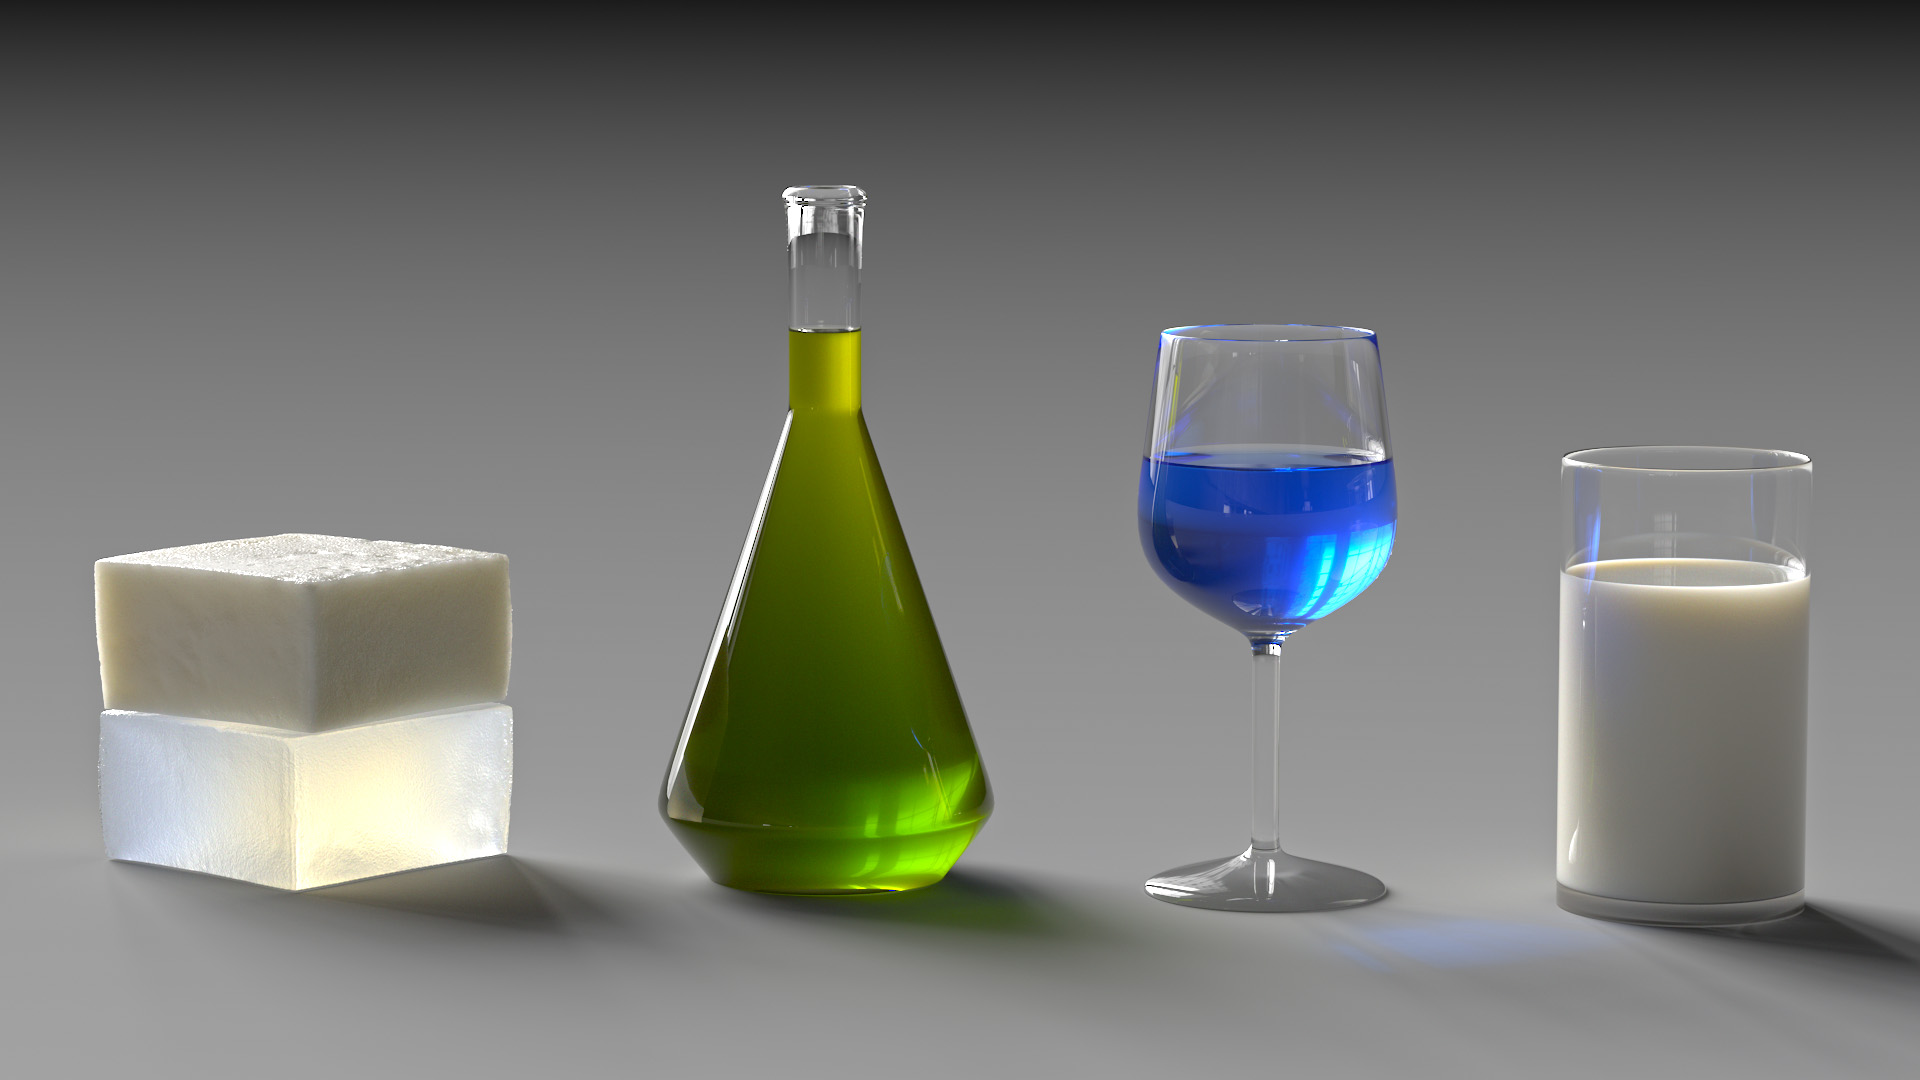
\includegraphics[scale=0.16]{trans.jpg}
  \end{figure}
}

\end{frame}


\section{BSSRDF}
\begin{frame}
  \frametitle{Light Transmission Models}
\only<1>{\begin{figure}[!ht]
    \centering
    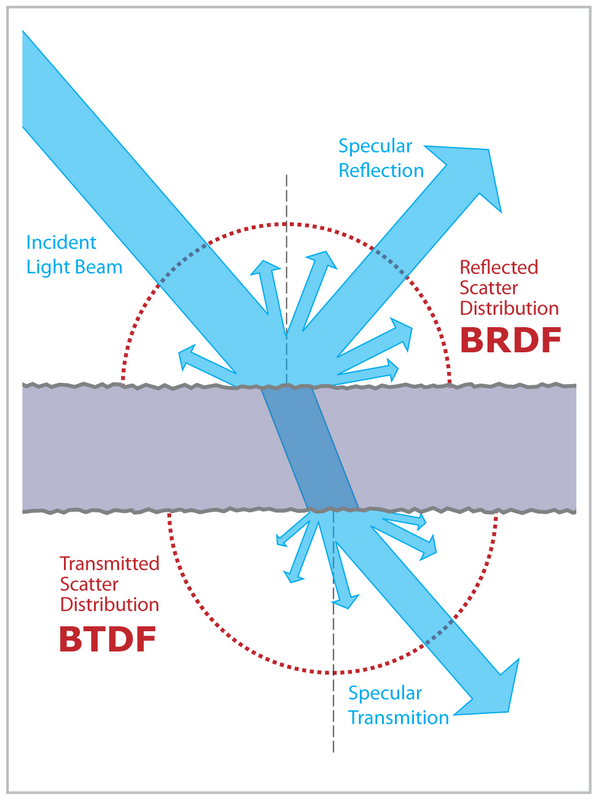
\includegraphics[scale=0.25]{bsdf.png}
  \end{figure}
}
\only<2>{
\begin{figure}[!ht]
    \centering
    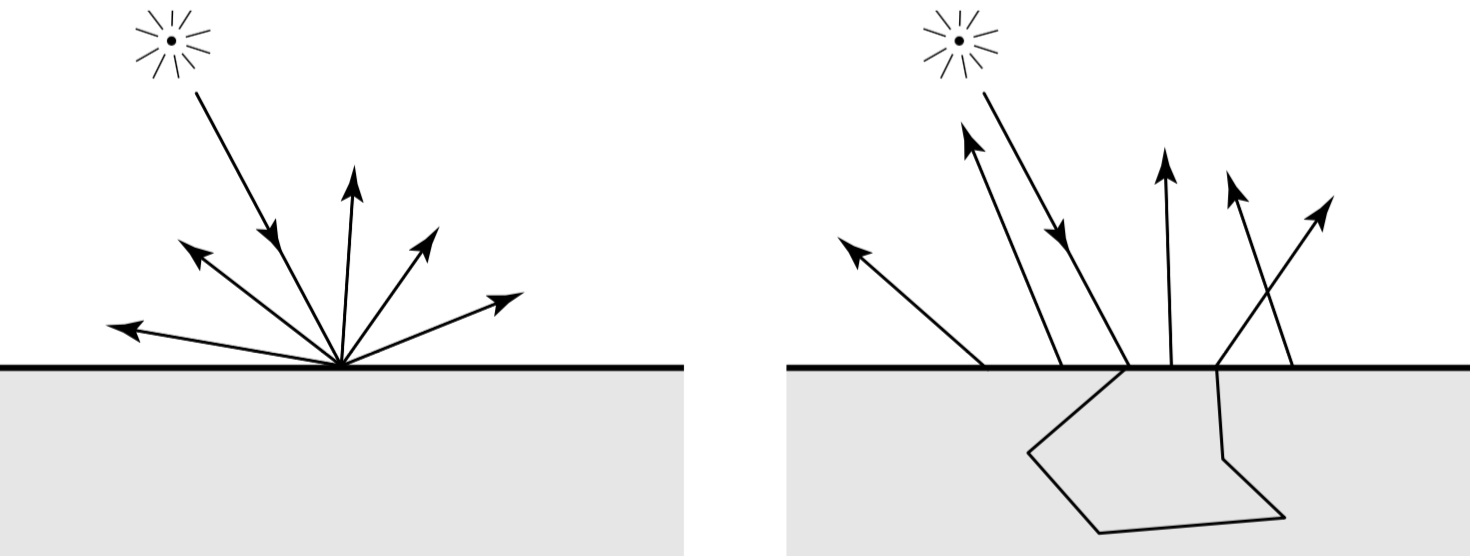
\includegraphics[scale=0.4]{bsdfbssrdf.png}
    \caption{Two models to describe the light transmission in
      translucent materials.}
  \end{figure}

}
\end{frame}





\begin{frame}
  \frametitle{BSSRDF Rendering}
Rendering translucent material takes a little bit more effort:

  \begin{align*}
\flux{o} &= \flux{e} + \flux{r} = \flux{e}\\
         & + \int_A\int_{2\pi}S(x_i, \vec{\omega_i}; x_o,
           \vec{\omega_o})L_i(\pmb{x}, \vec{\omega})(\vec{\omega}\cdot\vec{n})d\omega_idA
  \end{align*}

and

$$
S(x_i, \vec{\omega_i}; x_o, \vec{\omega_o})  = S_d(x_i,
\vec{\omega_i}; x_o, \vec{\omega_o}) +S^{(1)}(x_i, \vec{\omega_i};
x_o, \vec{\omega_o})
$$

where $S$ is BSSRDF. $S_d$ and $S^{(1)}$ are the{\bf  diffusion approximation} and
{\bf single scattering term}.

\end{frame}


\begin{frame}

\frametitle{Diffusion Approximation - Dipole}
  \begin{figure}[!ht]
    \centering
    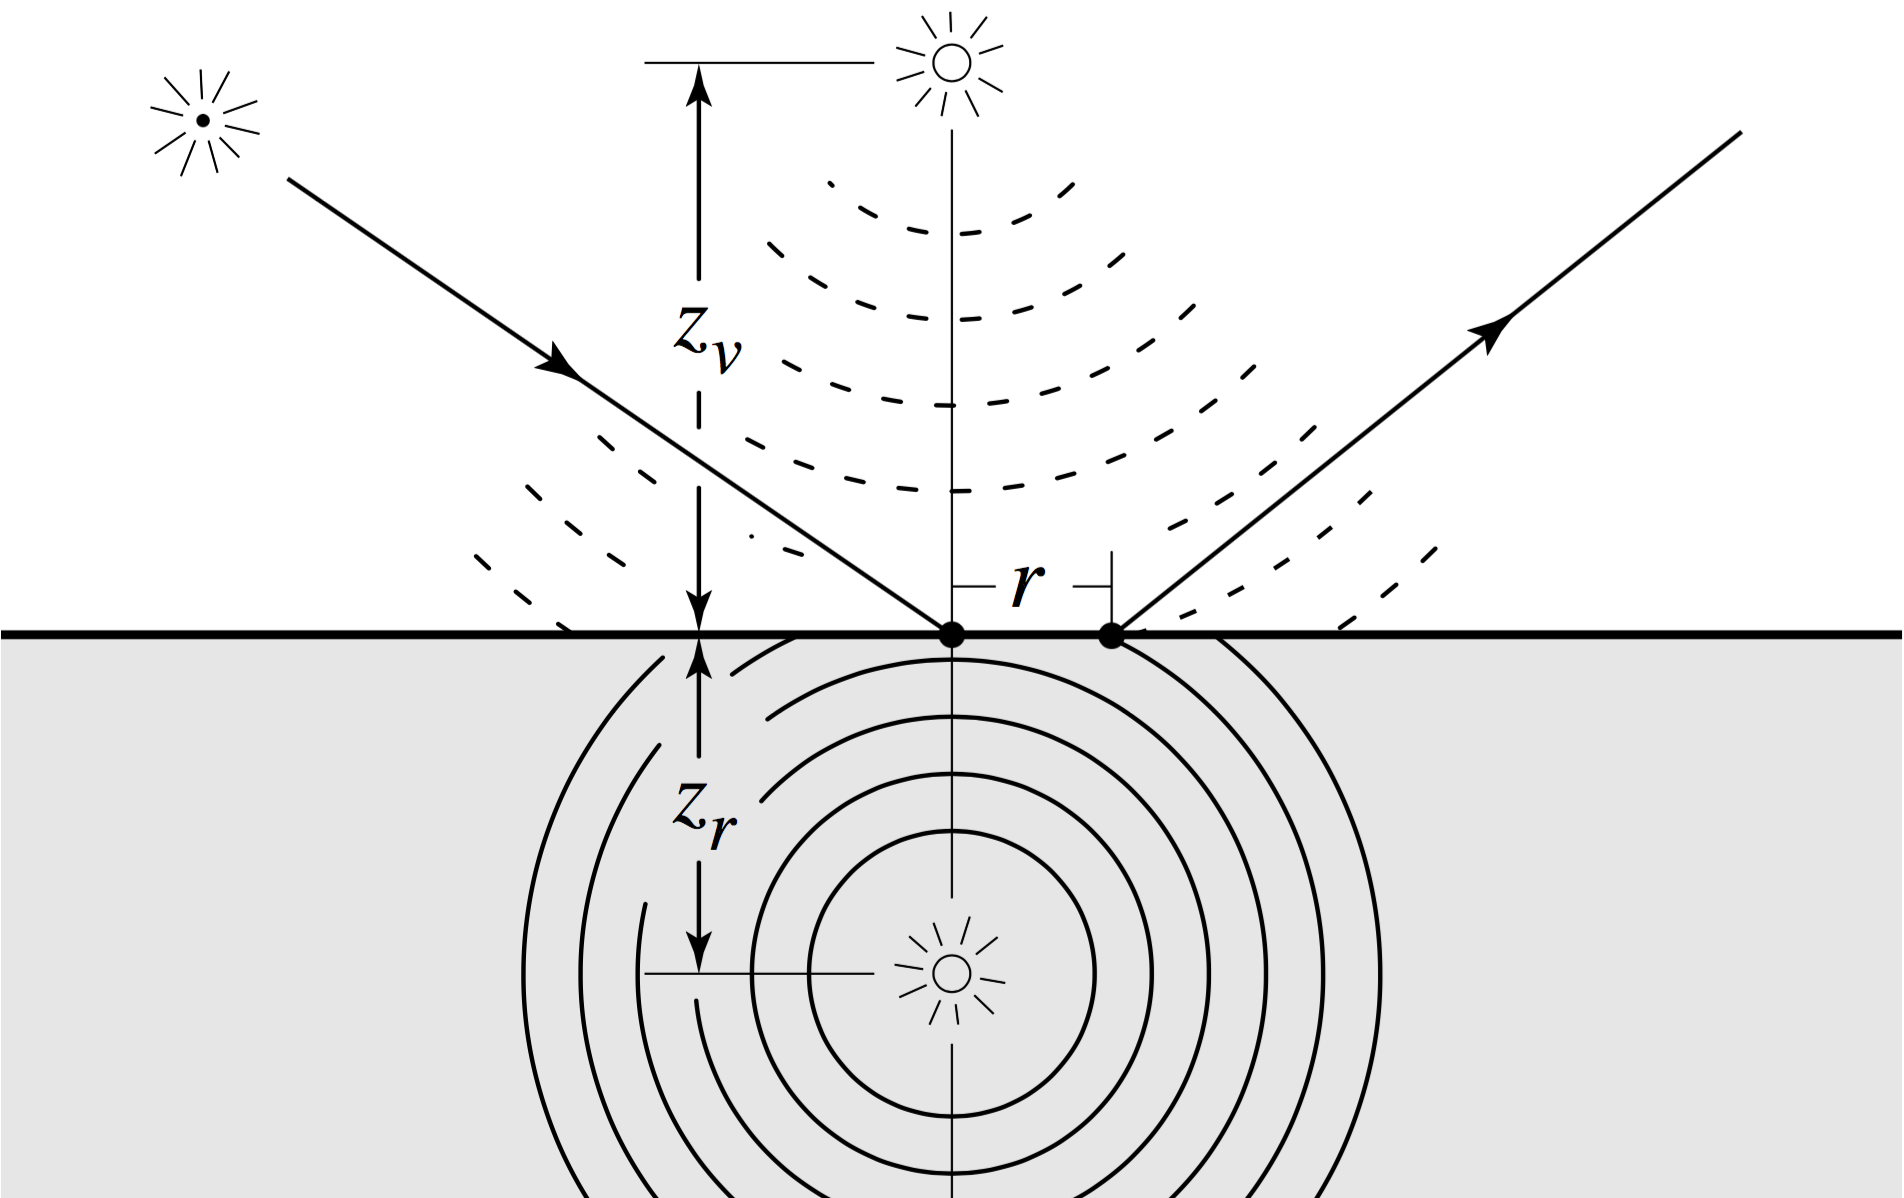
\includegraphics[scale=0.15]{di.png}
    \hspace{4mm}
    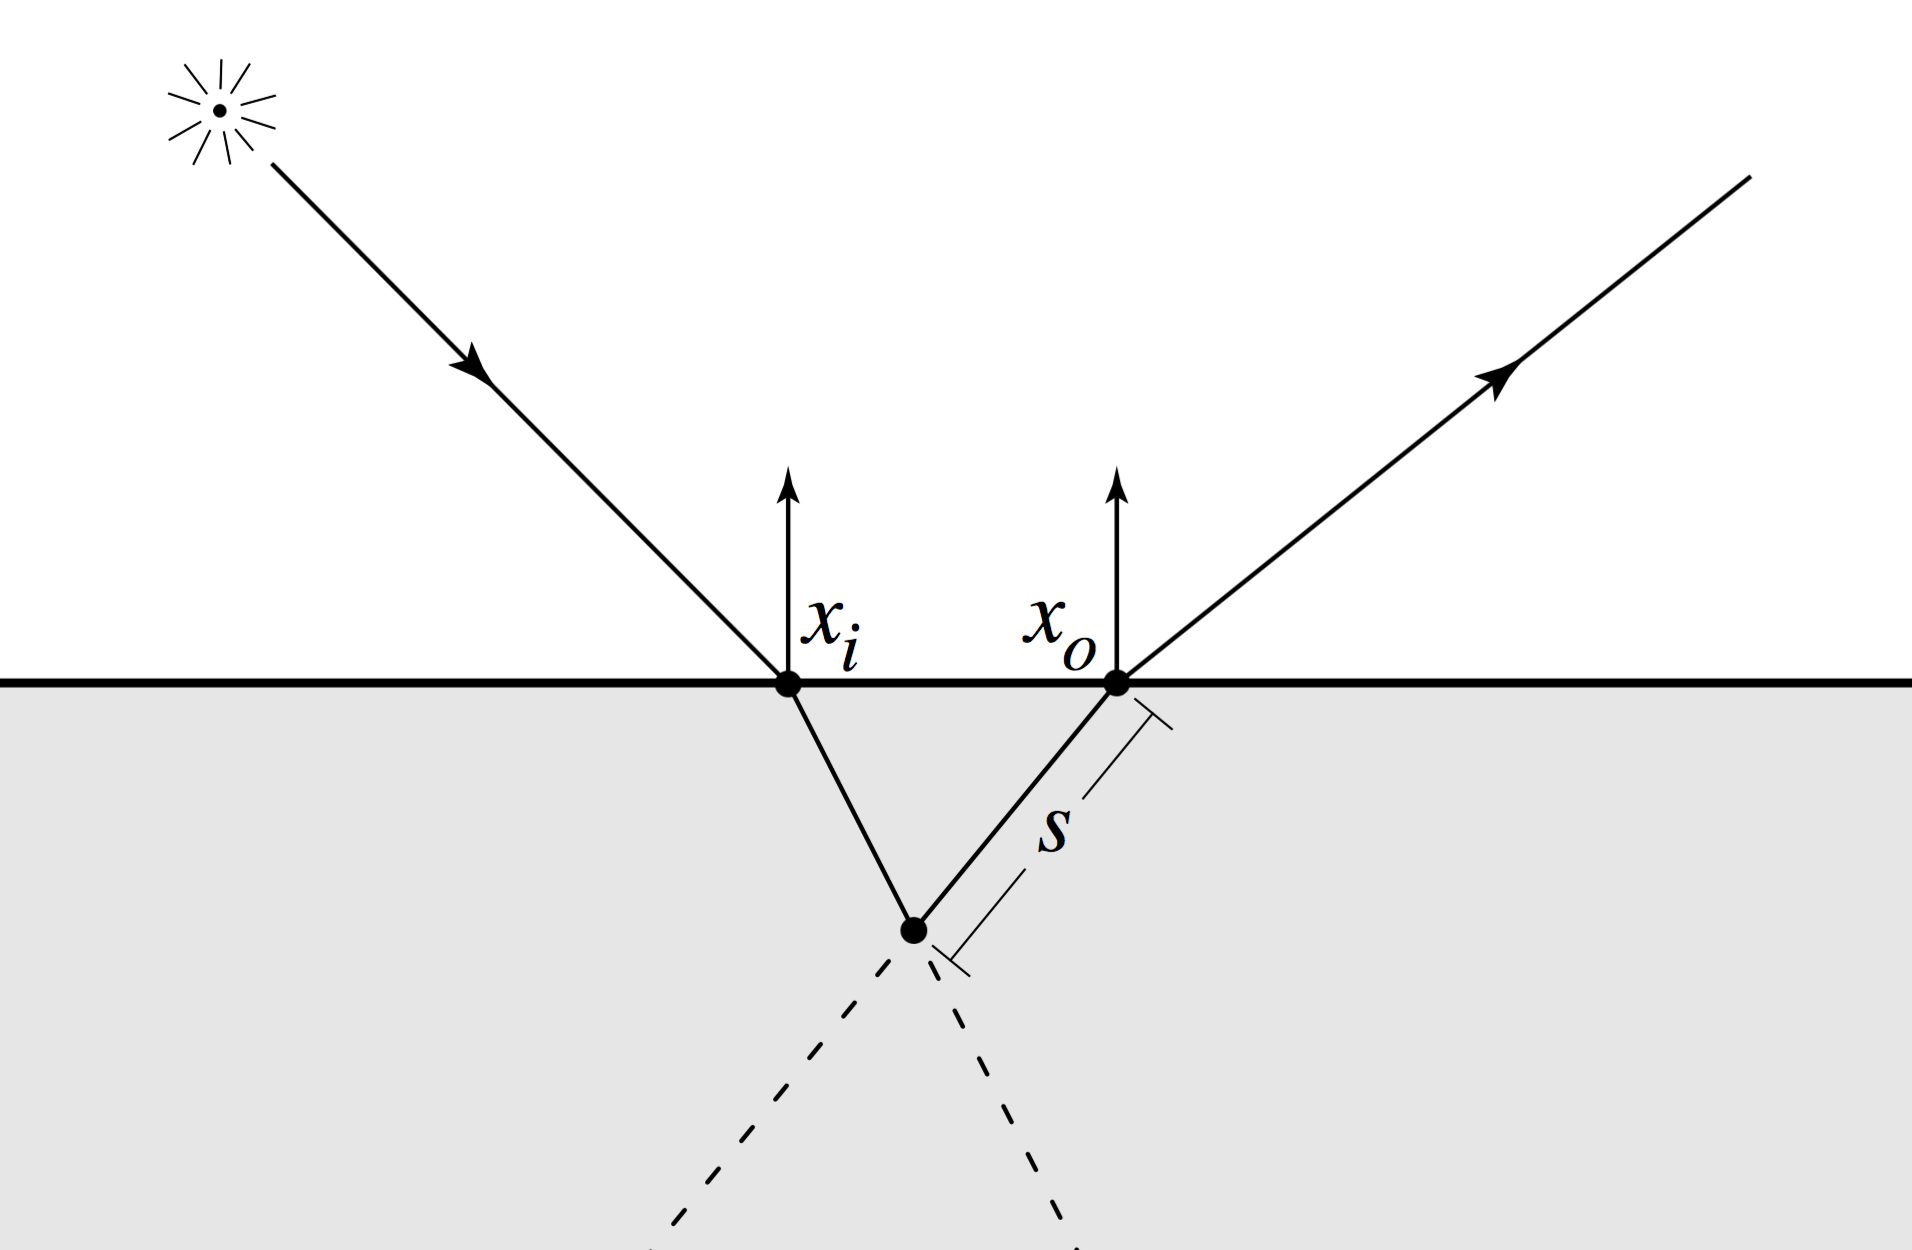
\includegraphics[scale=0.15]{single.png}
    \caption{A lot of math in the first graph. Single scattering occurs only when the refracted incoming and outgoing rays intersect.}
  \end{figure}
\end{frame}


\begin{frame}
  \frametitle{Photon Mapping - Engineering}
  \begin{itemize}
  \item Send photons to field, once intersecting with a surface, the
    incident(position and direction) will be stored in {\bf photon map};
  \item Actually 2 photon maps will be generated, one for caustics and
    one for SSS;
  \item Depends on the material, the action of the photon is processed
    with Monte Carlo method;
\item Then there should be optimizations, cause Monte Carlo is not
  graphic card friendly.
  \end{itemize}
\end{frame}




\section{Directional Dipole}

\begin{frame}
  \frametitle{Directional Dipole Model}
  \only<1>{\begin{figure}[!ht]
    \centering
    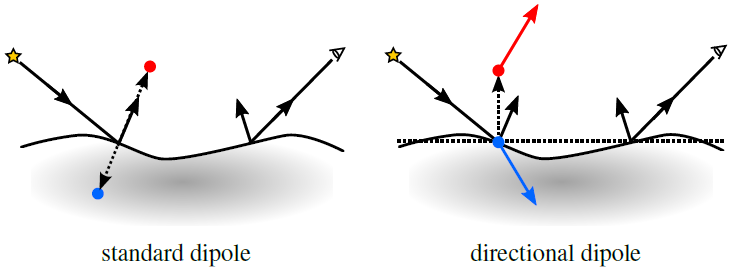
\includegraphics[scale=0.55]{dipoles.png}
  \end{figure}
}
\only<2>{
  \begin{figure}[!ht]
    \centering
    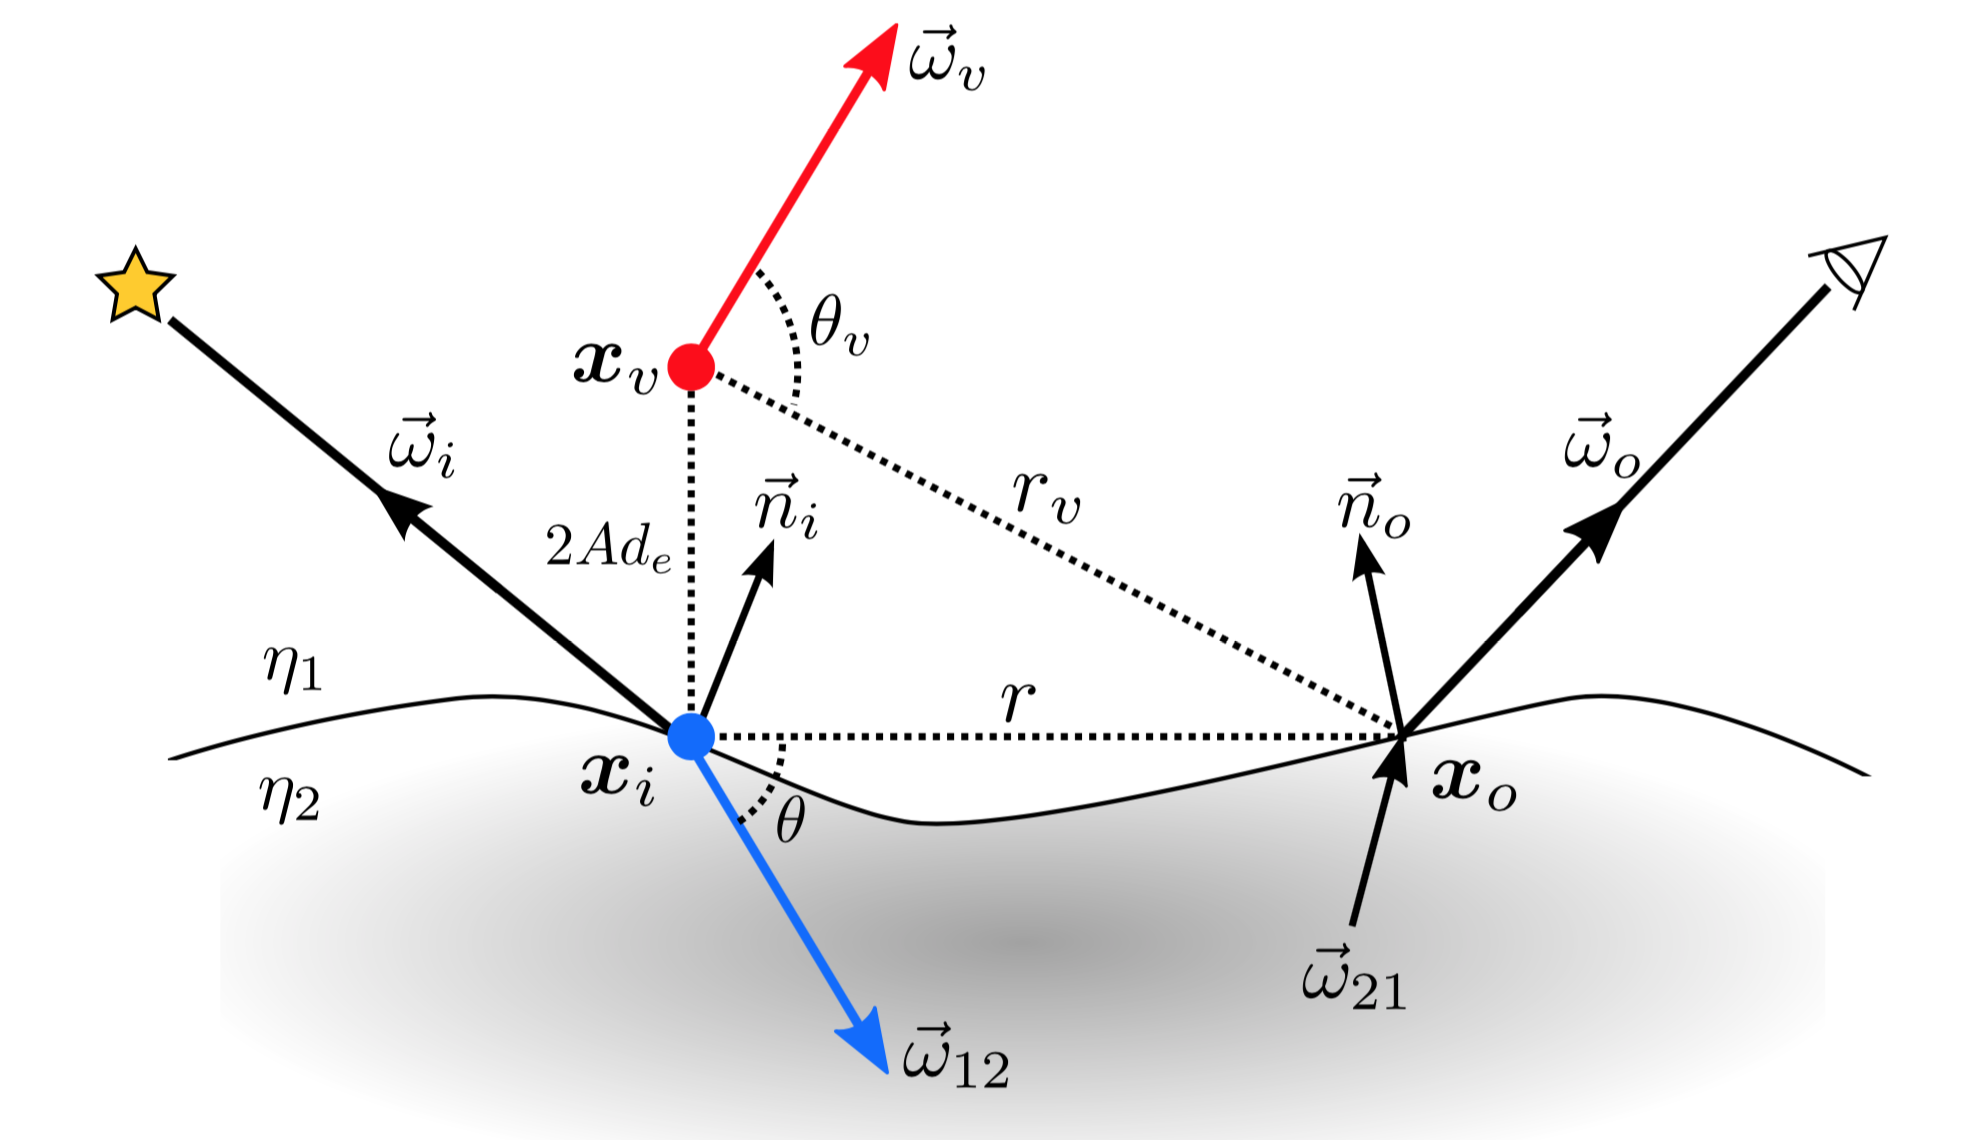
\includegraphics[scale=0.26]{direct.png}
  \end{figure}
And Diffusive part of BSSRDF in this paper is(a lot of math):
$$
S_d(\pmb{x_i}, \vec{\omega}; \pmb{x_o}) = S'_d(\pmb{x_o - x_i},
\vec{\omega}_{12}, d_r) - S'_d(\pmb{x_o - x_v}, \vec{\omega}_{v}, d_v)
$$

}
\end{frame}

\begin{frame}
  \frametitle{Some Comparisons}
  \only<1>{
    \begin{figure}[!ht]
      \centering
      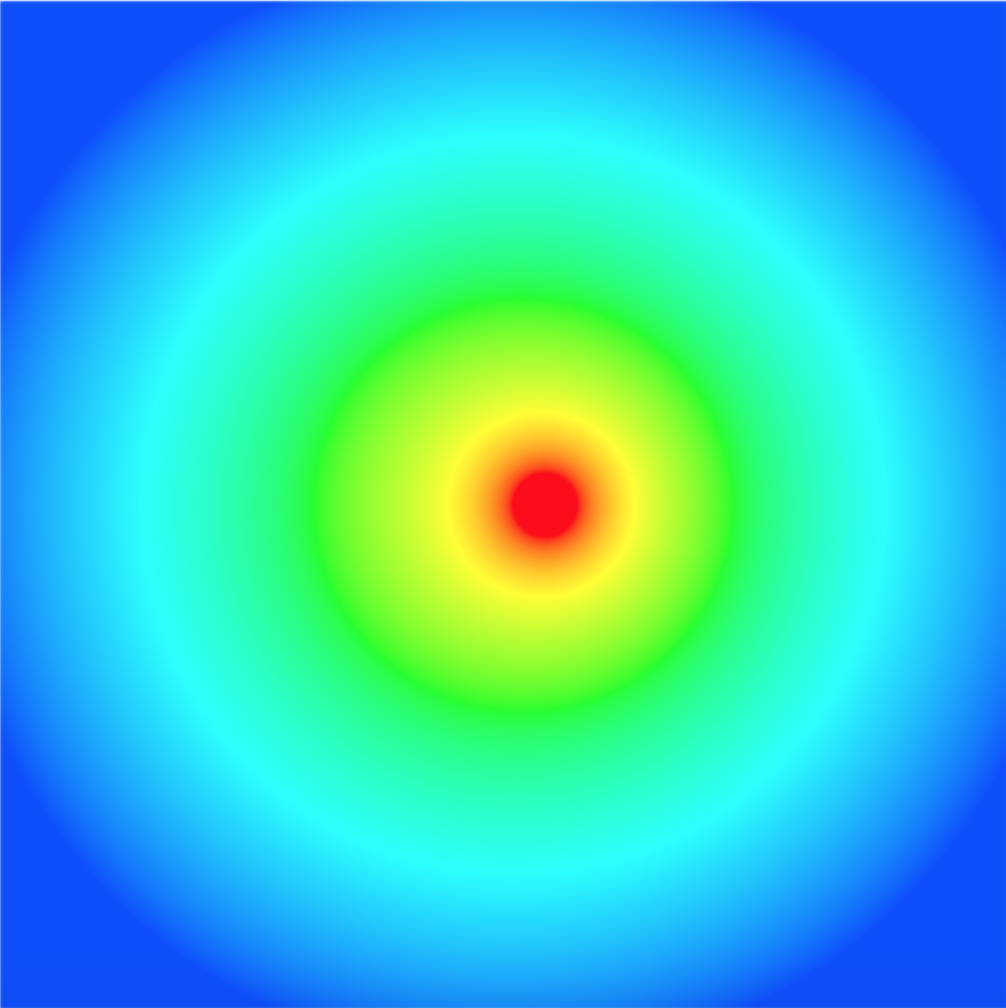
\includegraphics[scale=0.25]{so.png}
\hspace{4mm}
      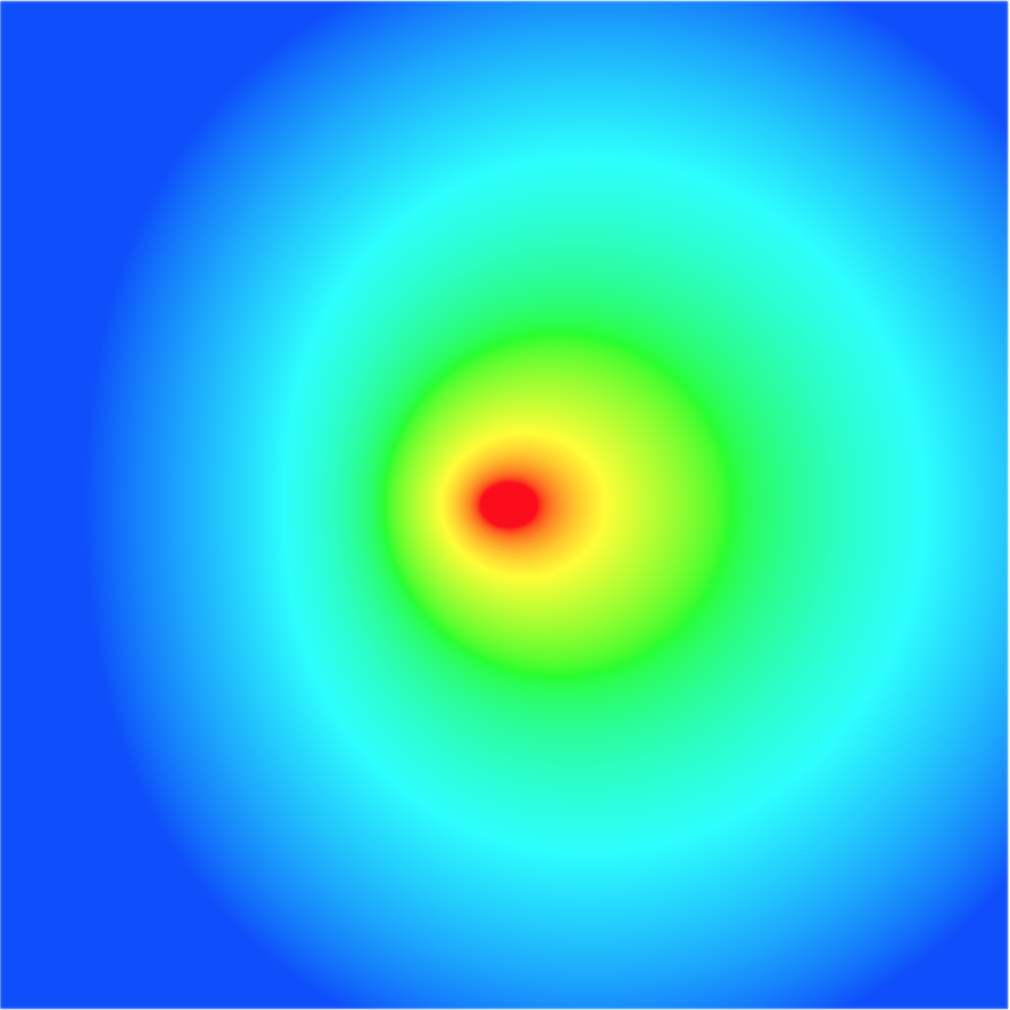
\includegraphics[scale=0.25]{sn.png}\\
    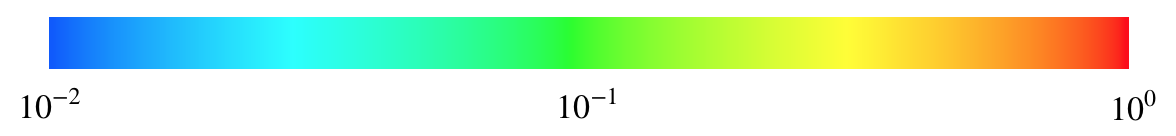
\includegraphics[scale=0.5]{bar.png}
      \caption{Diffuse reflectance due to approximate single
        scattering. Tested with Standard(left) and Directional Dipole. The
        incident angle is 45 degrees. }
    \end{figure}
  }
\only<2>{
\begin{figure}[!ht]
      \centering
      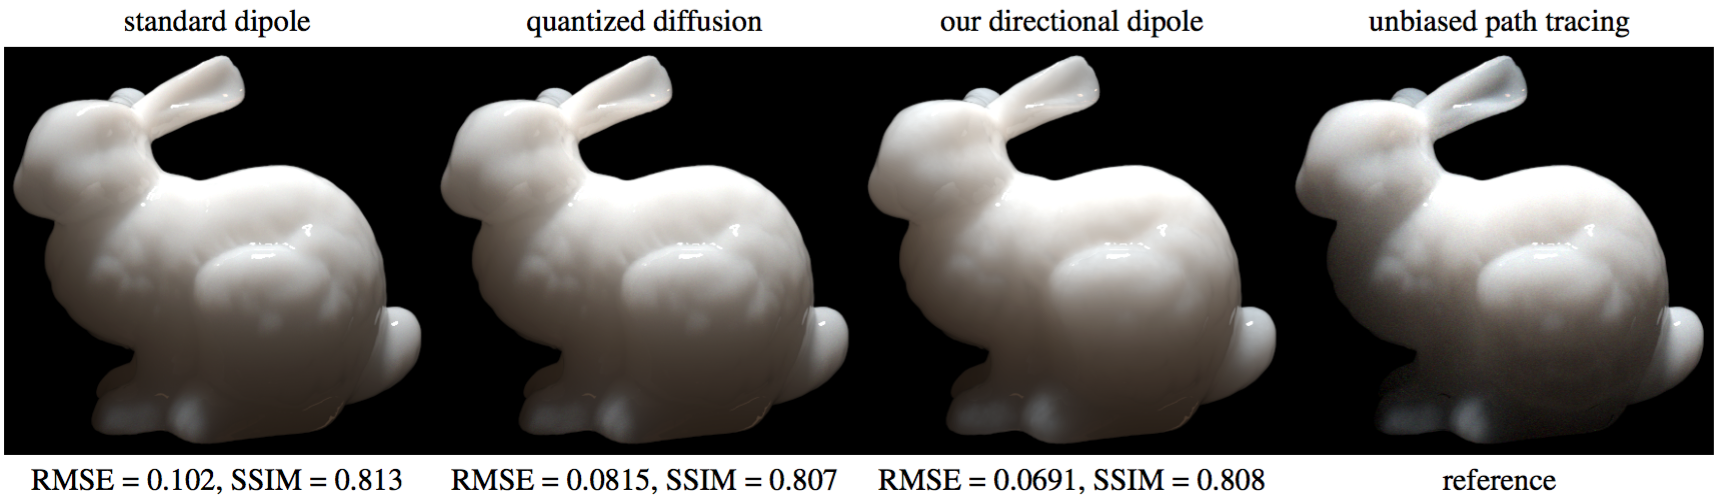
\includegraphics[scale=0.35]{stan.png}
      \caption{Comparison among different methods.}
    \end{figure}
}
\only<3>{
  \begin{itemize}
  \item No precomputation required;
  \item Single scattering does not need Monte Carlo simulation;
\item This whole thing is just to take the boundary into consideration actually.
  \end{itemize}
}
\end{frame}

\begin{frame}
  \frametitle{Basic Implementation}
  \only<1>{\begin{figure}[!ht]
    \centering
    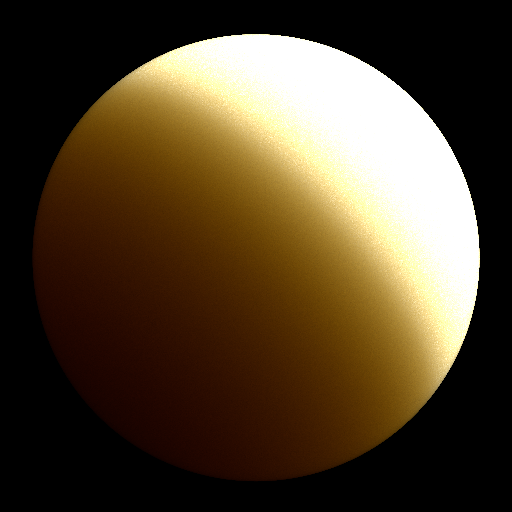
\includegraphics[scale=0.4]{render.png}
  \end{figure}
}
\only<2>{
\begin{figure}[!ht]
    \centering
    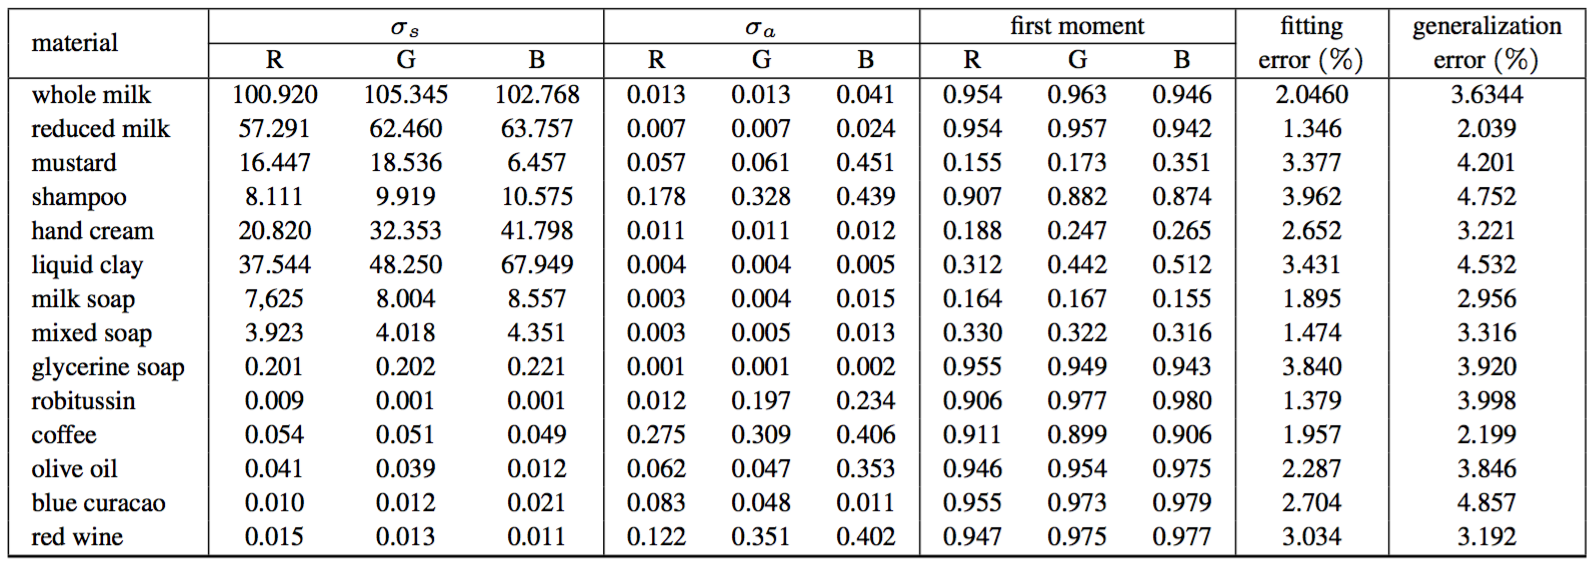
\includegraphics[scale=0.4]{supple.png}
  \end{figure}

}
\end{frame}
